% Provenance (never printed): cycle 2 "Questionner l'espace et le temps"
% (oceans, seas, continents on the globe) and "Questionner le monde de la
% matiere" (states of water in natural phenomena); see sources/book1/PROVENANCE.md.
% Book 1, grade 2, chapter 1.
\chapter{Water on Earth}\label{ch:g2:water-on-earth}

On the 7th of December 1972, three astronauts on their way to the Moon
turned their camera back towards the Earth. Their photograph became one of
the most famous pictures ever taken. Look at it. You can see white clouds,
a little brown and yellow land, the white ice at the bottom --- and blue,
blue everywhere. Seen from space, our planet is a blue planet.

\begin{omfigure}
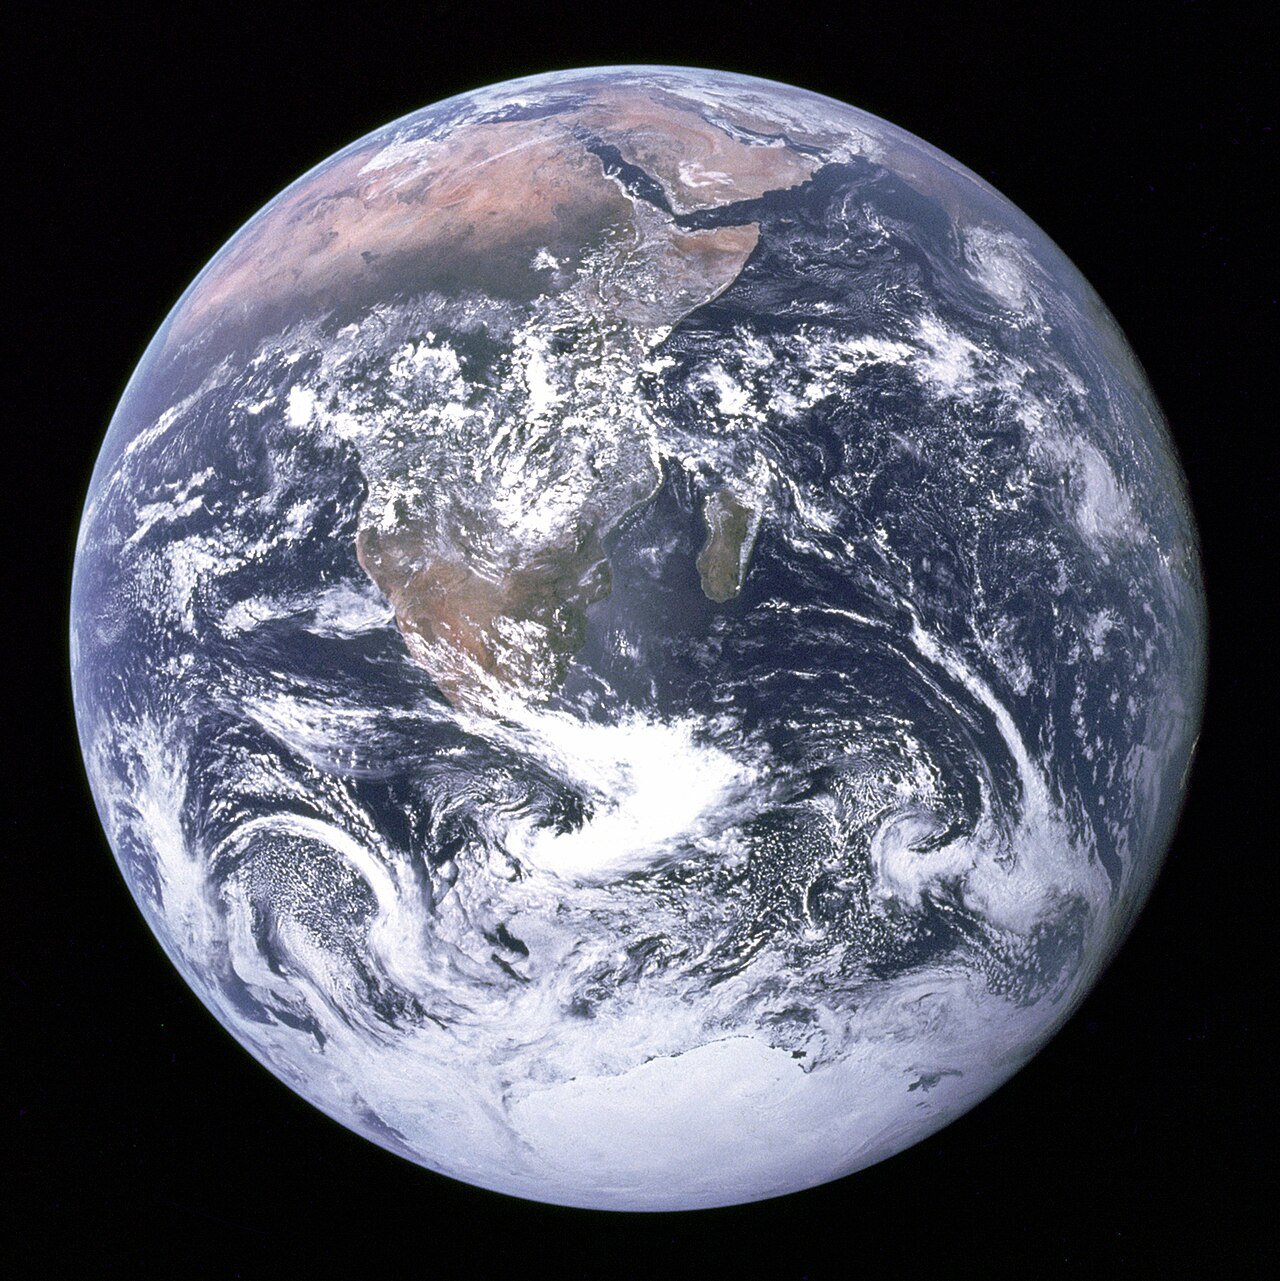
\includegraphics[width=0.5\linewidth]{images/book1/g2-nasa-blue-marble.jpg}

{\small The Earth photographed by the crew of Apollo~17, 7~December 1972.
We see Africa, Arabia at the top, and the ice of Antarctica at the bottom.
Photograph: NASA (public domain).}
\end{omfigure}

\begin{recall}
Water can be a solid (ice), a liquid, or a gas that we cannot see (water
vapour). Liquid water left in the sun slowly turns into vapour: it
evaporates. When the vapour cools, it turns back into tiny drops: it
condenses. You have met these changes in the physics books. In a \omterm{def:g1:landscapes-around-us:landscape}{landscape},
water flows in \omterm{def:g1:landscapes-around-us:water}{rivers} and lies in \omterm{def:g1:landscapes-around-us:water}{lakes} (\cref{ch:g1:landscapes-around-us}).
\end{recall}

\section{The blue planet}

Most of the Earth is covered by water. Imagine the whole surface of the
Earth cut into 100 equal squares. If we colour in blue every square that
is covered by \omterm{def:g2:water-on-earth:ocean}{sea}, we colour 71 squares. Only 29 squares are land.

\begin{omfigure}
\begin{tikzpicture}
  \begin{axis}[hide axis, width=7.2cm, height=7.2cm, xmin=-0.5, xmax=9.5,
      ymin=-0.5, ymax=9.5, axis equal image, scale only axis,
      clip=false]
    \addplot[scatter, only marks, mark=square*, mark size=9.2pt,
      scatter/classes={0={fill=green!45!omLithAlluv, draw=black!40},
                       1={fill=omSea!80!blue, draw=black!40}},
      point meta=explicit symbolic]
      table[x=col, y=row, meta=blue] {figdata/out/grade-2-ocean_fraction-grid.dat};
  \end{axis}
\end{tikzpicture}

{\small If the Earth's surface were cut into 100 equal squares, 71 would be
\omterm{def:g2:water-on-earth:ocean}{sea} (blue) and 29 would be land (green). Computed from a map of the whole
Earth's relief (NOAA ETOPO1).}
\label{fig:g2:water-on-earth:grid}
\end{omfigure}
% ledger: data:etopo1, wss:ocean-cover (71 % computed in figdata/grade-2/ocean_fraction.py)

The great stretches of \omterm{def:g2:water-on-earth:salt-fresh}{salt water} that cover most of the Earth have names.

\begin{definition}[Ocean and sea]\label{def:g2:water-on-earth:ocean}
An \emph{ocean}\index{ocean} is one of the very large stretches of \omterm{def:g2:water-on-earth:salt-fresh}{salt
water} that cover most of the Earth and lie between the continents. A
\emph{sea}\index{sea} is a smaller stretch of \omterm{def:g2:water-on-earth:salt-fresh}{salt water}, usually at the
edge of an ocean and partly closed in by land.
\end{definition}

All the \omterm{def:g2:water-on-earth:ocean}{oceans} are joined to one another: a boat could sail from any \omterm{def:g2:water-on-earth:ocean}{ocean}
to any other without crossing land. Their names, and where they lie on a
globe, are in \cref{ch:g3:continents-and-oceans}.

\begin{omfigure}
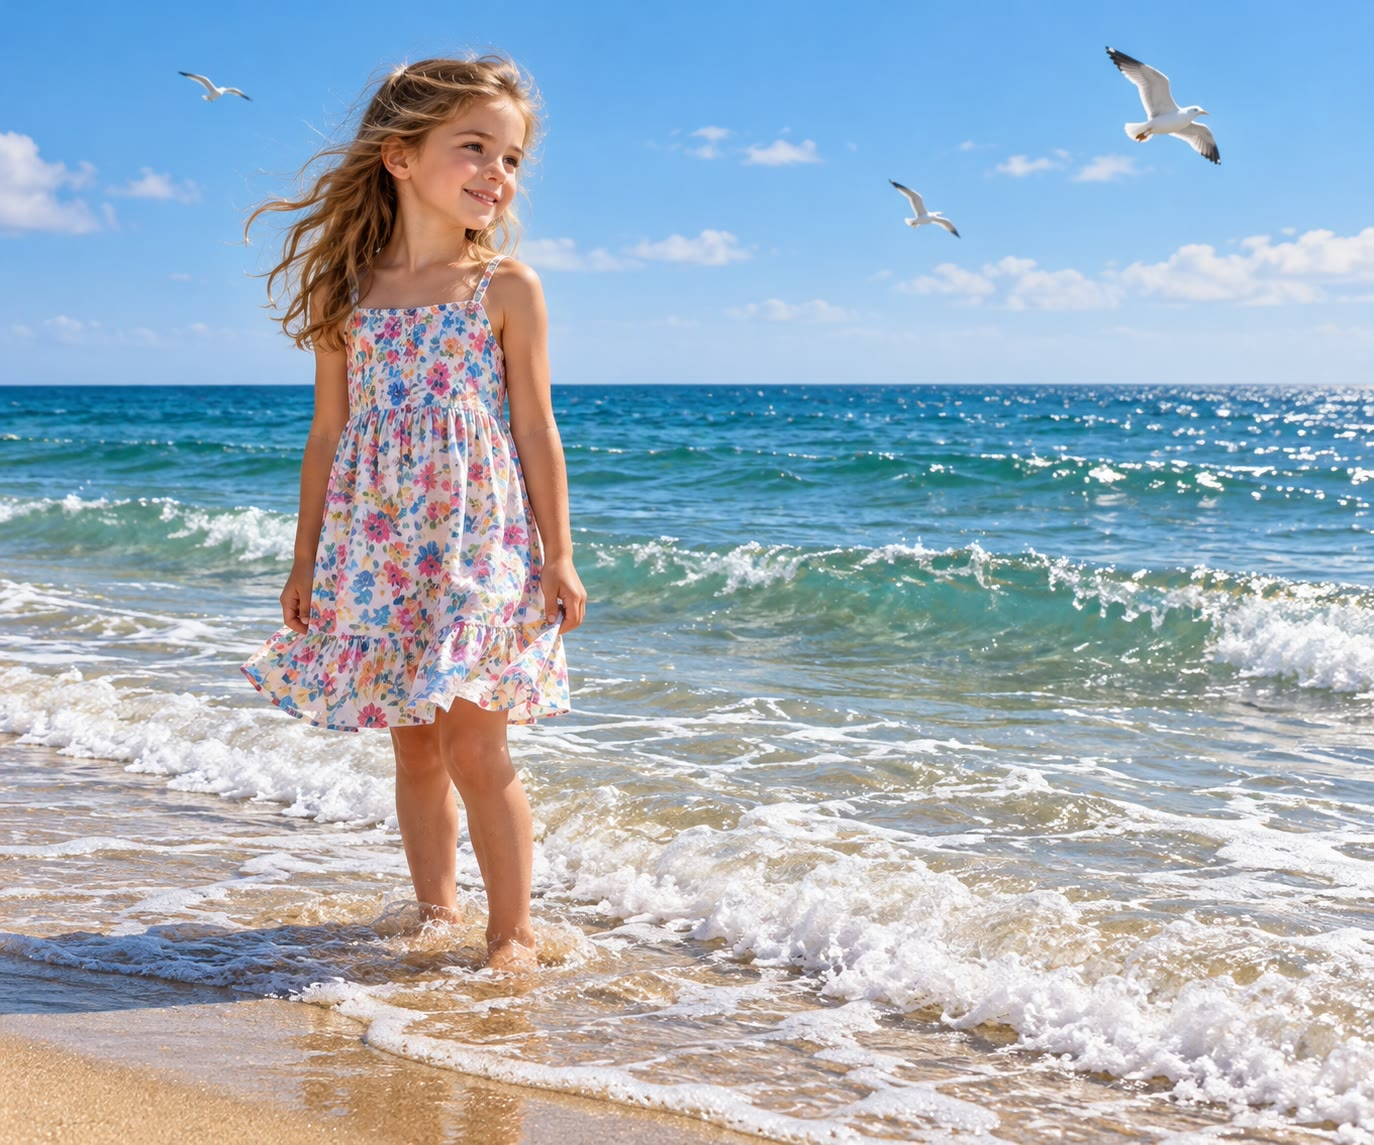
\includegraphics[width=0.62\linewidth]{images/book1/ai/g2-beach-sea.jpg}

{\small At the edge of the \omterm{def:g2:water-on-earth:ocean}{sea}. The water goes on, much farther than the
eye can see.}
\end{omfigure}

\section{Salt water and fresh water}

If you have ever swallowed a mouthful of \omterm{def:g2:water-on-earth:ocean}{sea} water while swimming, you
know: it tastes very salty. The water of \omterm{def:g1:landscapes-around-us:water}{rivers} and \omterm{def:g1:landscapes-around-us:water}{lakes} does not.

\begin{definition}[Salt water and fresh water]\label{def:g2:water-on-earth:salt-fresh}
\emph{Salt water}\index{salt water} has a lot of salt dissolved in it: it is
the water of the \omterm{def:g2:water-on-earth:ocean}{oceans} and the \omterm{def:g2:water-on-earth:ocean}{seas}. \emph{Fresh water}\index{fresh water}
has very little salt: it is the water of rain, of most \omterm{def:g1:landscapes-around-us:water}{rivers} and \omterm{def:g1:landscapes-around-us:water}{lakes}, of
the ice and the snow, and of springs.
\end{definition}

\begin{example}[How salty is the sea?]\label{ex:g2:water-on-earth:salty}
% ledger: nos:salinity
In a bottle holding one kilogram of \omterm{def:g2:water-on-earth:ocean}{sea} water --- about one litre --- there
are about 35 grams of salt. If we let all the water evaporate, the salt
stays behind as white crystals at the bottom. That is how \omterm{def:g2:water-on-earth:ocean}{sea} salt is made
in salt marshes by the \omterm{def:g2:water-on-earth:ocean}{sea}, where the sun and the wind slowly dry out
shallow pools of \omterm{def:g2:water-on-earth:ocean}{sea} water.
\end{example}

\begin{omfigure}
\begin{minipage}[b]{0.49\linewidth}\centering
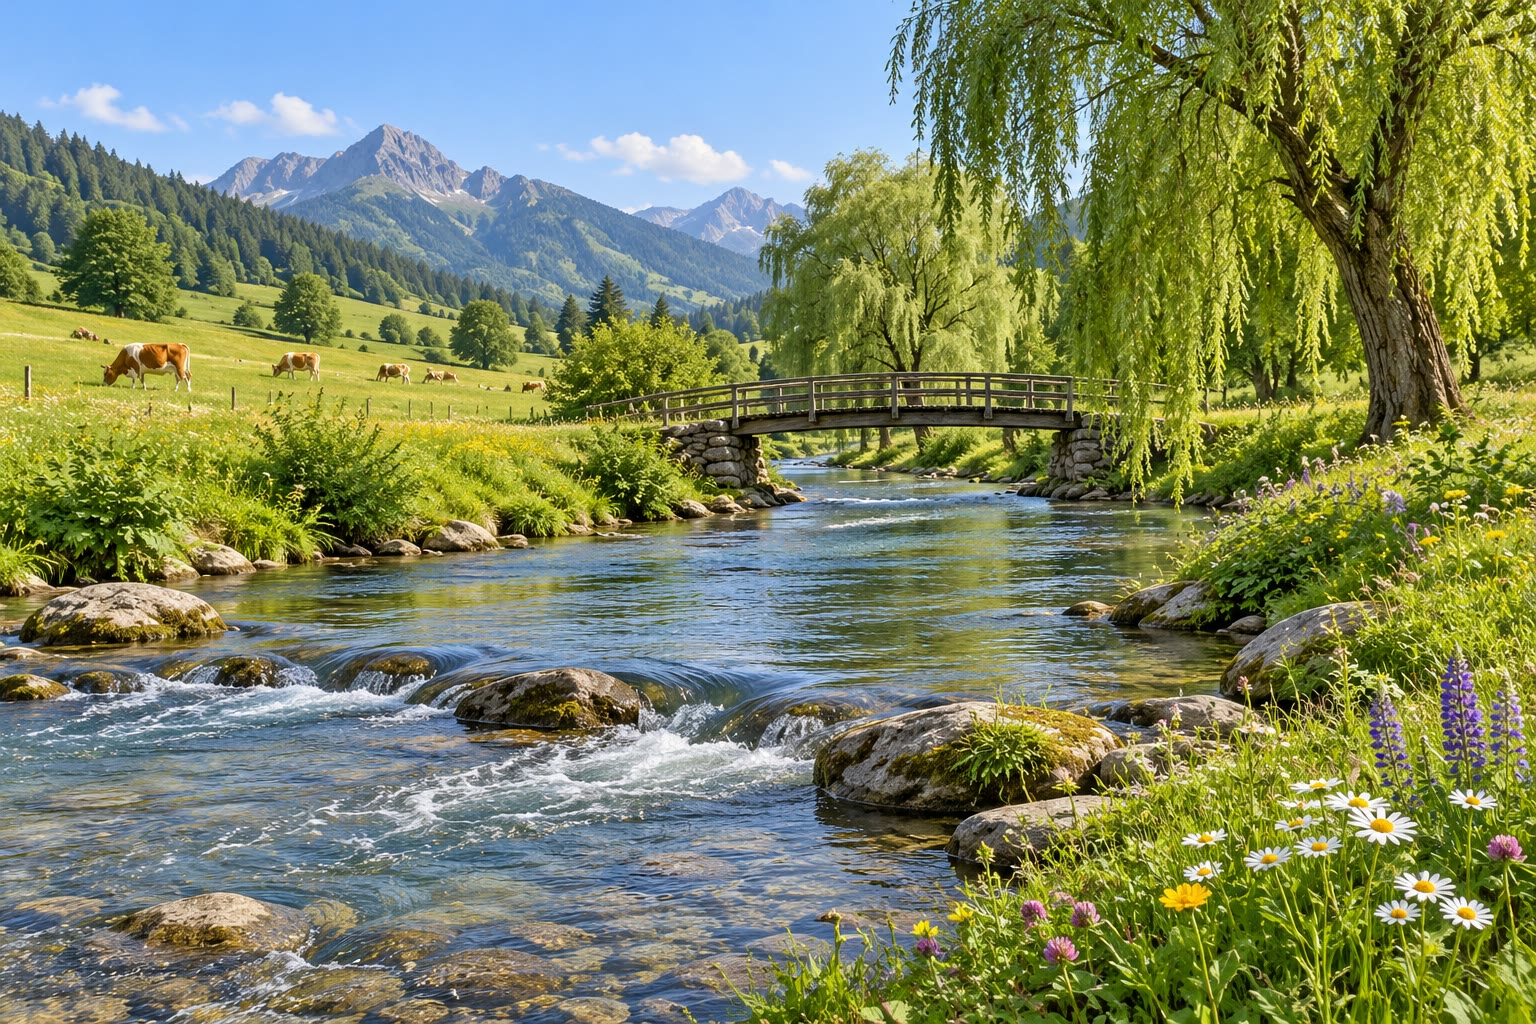
\includegraphics[width=\linewidth]{images/book1/ai/g2-river-meadow.jpg}

{\small \omterm{def:g2:water-on-earth:salt-fresh}{Fresh water}: a \omterm{def:g1:landscapes-around-us:water}{river}.}
\end{minipage}\hfill
\begin{minipage}[b]{0.49\linewidth}\centering
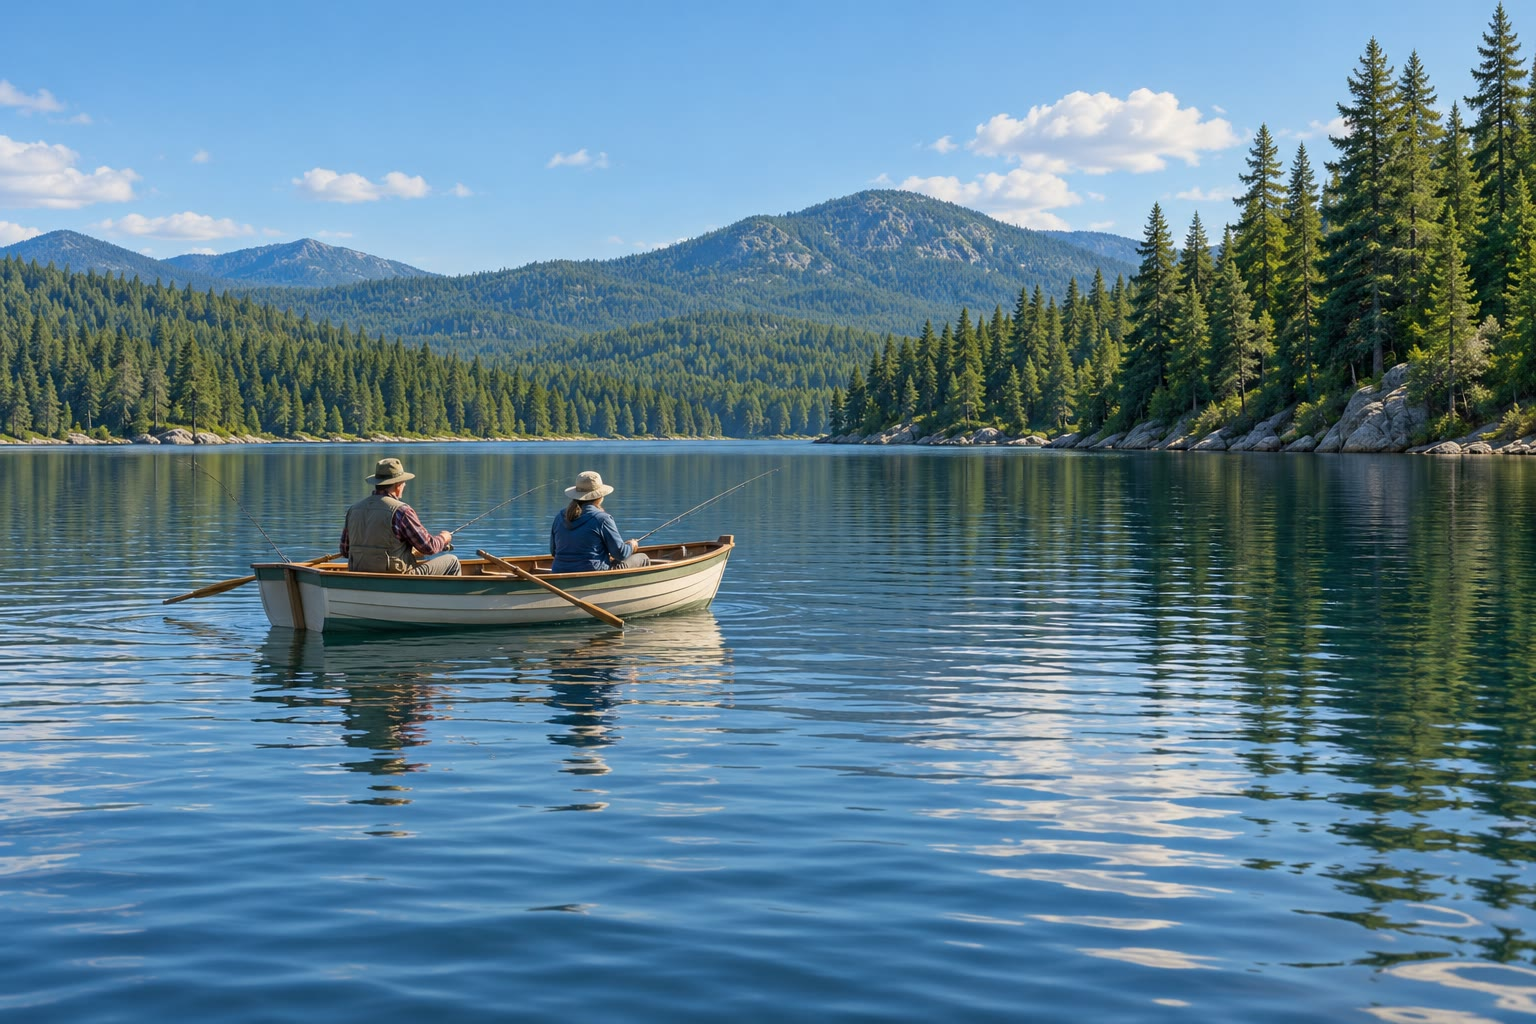
\includegraphics[width=\linewidth]{images/book1/ai/g2-lake-boat.jpg}

{\small \omterm{def:g2:water-on-earth:salt-fresh}{Fresh water}: a \omterm{def:g1:landscapes-around-us:water}{lake}.}
\end{minipage}
\end{omfigure}

\begin{remark}[We cannot drink sea water]\label{rem:g2:water-on-earth:drink}
People and land animals cannot drink \omterm{def:g2:water-on-earth:ocean}{sea} water: there is too much salt in
it, and drinking it makes the body lose water instead of gaining it.
Sailors far out at \omterm{def:g2:water-on-earth:ocean}{sea}, surrounded by water, have always had to carry their
\omterm{def:g2:water-on-earth:salt-fresh}{fresh water} with them.
\end{remark}

\section{Where is all the water?}

\omterm{def:g2:water-on-earth:salt-fresh}{Fresh water} is not only in \omterm{def:g1:landscapes-around-us:water}{rivers} and \omterm{def:g1:landscapes-around-us:water}{lakes}. A lot of it is frozen: in the
great white ice of Antarctica and Greenland, and on the high \omterm{def:g1:landscapes-around-us:landform}{mountains}.
And a lot of it is hidden under our feet, in the ground, where it fills the
tiny spaces between grains of sand and cracks in the rock.

\begin{omfigure}
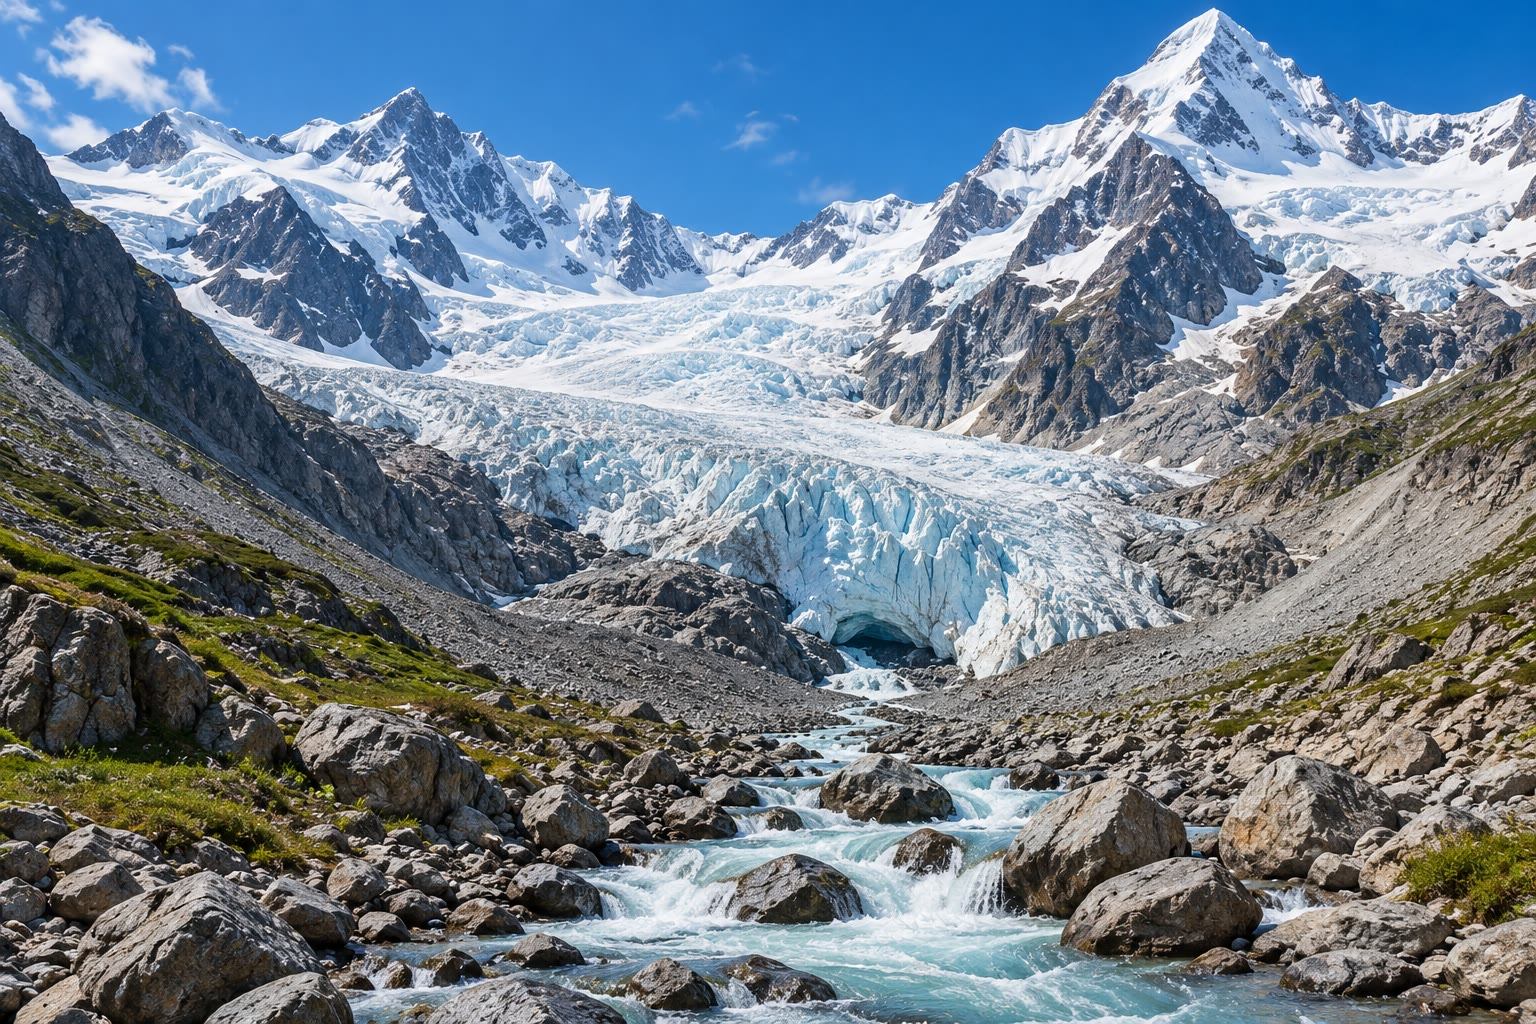
\includegraphics[width=0.62\linewidth]{images/book1/ai/g2-snowy-mountains.jpg}

{\small High \omterm{def:g1:landscapes-around-us:landform}{mountains} keep \omterm{def:g2:water-on-earth:salt-fresh}{fresh water} as snow and ice all year long. In
summer some of it melts and feeds the streams.}
\end{omfigure}

Imagine that we could pour all the water of the Earth into 100 buckets of
the same size. How many buckets would each kind of water fill?

\begin{omfigure}
\begin{tikzpicture}
  \begin{axis}[hide axis, width=7.2cm, height=7.2cm, xmin=-0.5, xmax=9.5,
      ymin=-0.5, ymax=9.5, axis equal image, scale only axis, clip=false]
    \addplot[scatter, only marks, mark=*, mark size=8pt,
      scatter/classes={0={fill=omSea!80!blue, draw=black!40},
                       1={fill=white, draw=black!60},
                       2={fill=brown!55, draw=black!40}},
      point meta=explicit symbolic]
      table[x=col, y=row, meta=kind] {figdata/out/grade-2-water_shares.dat};
  \end{axis}
  \begin{scope}[shift={(7.9,5.6)}, font=\small]
    \fill[omSea!80!blue, draw=black!40] (0,0) circle (0.2);
    \node[anchor=west] at (0.35,0) {salt water of the oceans: 96 buckets};
    \fill[white, draw=black!60] (0,-0.7) circle (0.2);
    \node[anchor=west] at (0.35,-0.7) {ice and snow: 2 buckets};
    \fill[brown!55, draw=black!40] (0,-1.4) circle (0.2);
    \node[anchor=west] at (0.35,-1.4) {water under the ground: 2 buckets};
  \end{scope}
\end{tikzpicture}

{\small All the water of the Earth in 100 buckets. The \omterm{def:g1:landscapes-around-us:water}{rivers}, the \omterm{def:g1:landscapes-around-us:water}{lakes},
the clouds and the water of all living things together would not fill even
one bucket. Numbers from the U.S. Geological Survey.}
\label{fig:g2:water-on-earth:buckets}
\end{omfigure}
% ledger: wss:water-shares (rounded to 100 buckets in figdata/grade-2/water_shares.py)

\begin{proposition}[Most of the Earth's water is salty]\label{prop:g2:water-on-earth:most-salty}
% ledger: wss:water-shares
Out of 100 buckets of all the water on Earth, 96 are the \omterm{def:g2:water-on-earth:salt-fresh}{salt water} of the
\omterm{def:g2:water-on-earth:ocean}{oceans}. The \omterm{def:g2:water-on-earth:salt-fresh}{fresh water} we drink is only a very small part of all the
water: most of it is frozen in the ice, or hidden under the ground.
\end{proposition}

\section{Where does the rain go?}

When it rains, the water does not stay where it falls. Watch the yard of
the school after a shower: some water runs over the ground into the
gutters, some soaks into the soil of the flower beds, and puddles slowly
disappear as the sun comes back.

\begin{omfigure}
\begin{tikzpicture}[x=1cm, y=1cm, font=\small]
  % sky, sea, land
  \fill[ocBlue!6] (0,0) rectangle (12,5.6);
  \fill[omSea] (8.6,0) rectangle (12,0.9);
  \fill[green!30!omLithAlluv] (0,0) -- (0,2.4) .. controls (2,2.6) and (3,2.0) .. (4.5,1.6)
     .. controls (6,1.2) and (7.5,1.0) .. (8.6,0.9) -- (8.6,0) -- cycle;
  % ground below the surface
  \fill[brown!25] (0,0) rectangle (8.6,0.6);
  % river
  \draw[omSea!70!blue, line width=2.4pt] (1.6,2.45) .. controls (3.5,2.0) and (6,1.15) .. (8.6,0.95);
  % cloud and rain
  \pic at (2.2,4.0) {puffycloud};
  \foreach \x in {1.4,1.8,2.2,2.6,3.0}
    \draw[omWxRain, line width=0.8pt] (\x,3.7) -- (\x-0.15,3.1);
  \pic at (9.6,4.3) {puffycloud};
  % arrows
  \draw[omWxRain, line width=1.1pt, -{Stealth[length=2.5mm]}] (3.3,2.15) -- (3.3,0.6);
  \node[anchor=west, align=left, font=\scriptsize] at (3.4,1.0) {some soaks\\into the ground};
  \draw[omWxRain, line width=1.1pt, -{Stealth[length=2.5mm]}] (5.4,1.55) -- (7.6,1.15);
  \node[align=center, font=\scriptsize] at (6.2,2.05) {some runs into a river,\\and the river runs to the sea};
  \draw[black!50, line width=1.1pt, densely dashed, -{Stealth[length=2.5mm]}] (10.2,1.1) .. controls (10.4,2.4) and (10.1,3.2) .. (9.8,3.85);
  \node[align=left, anchor=west, font=\scriptsize] at (10.45,2.4) {water\\evaporates};
  \draw[black!50, line width=1.1pt, densely dashed, -{Stealth[length=2.5mm]}] (8.45,4.35) -- (3.6,4.3);
  \node[font=\scriptsize, above] at (6.0,4.35) {the wind carries the clouds};
  \node[font=\scriptsize] at (10.4,0.45) {sea};
  \node[font=\scriptsize, anchor=west] at (0.2,3.25) {rain};
\end{tikzpicture}

{\small Where the rain goes. The water that rises from the \omterm{def:g2:water-on-earth:ocean}{sea} and from the
land as vapour makes new clouds, and the clouds bring new rain.}
\label{fig:g2:water-on-earth:rain}
\end{omfigure}

\begin{method}[Following a drop of rain]\label{met:g2:water-on-earth:drop}
To follow a drop of rain, ask three questions in turn:
\begin{enumerate}
  \item Where does it fall: on the \omterm{def:g2:water-on-earth:ocean}{sea}, on a roof, on the soil, on a
        \omterm{def:g1:landscapes-around-us:landform}{mountain}?
  \item Does it soak into the ground, run off over the surface, or freeze
        into ice?
  \item Where does it go next: into a \omterm{def:g1:landscapes-around-us:water}{river}, a \omterm{def:g1:landscapes-around-us:water}{lake}, the \omterm{def:g2:water-on-earth:ocean}{sea}, the ground,
        or back into the air?
\end{enumerate}
In the end, every drop comes back to the \omterm{def:g2:water-on-earth:ocean}{sea} or to the air, and the
journey starts again.
\end{method}

\begin{example}[A drop on the mountain]\label{ex:g2:water-on-earth:mountain}
A drop of rain falls as snow on a high \omterm{def:g1:landscapes-around-us:landform}{mountain} in winter. It stays there,
frozen, until the warm days of summer. Then it melts, runs down into a
\omterm{def:g1:landscapes-around-us:landform}{mountain} stream, joins a \omterm{def:g1:landscapes-around-us:water}{river}, and the \omterm{def:g1:landscapes-around-us:water}{river} carries it to the \omterm{def:g2:water-on-earth:ocean}{sea}. One
sunny day the drop evaporates from the \omterm{def:g2:water-on-earth:ocean}{sea} and rises into the air, where it
becomes part of a new cloud.
\end{example}

\section{Exercises}

\begin{exercise}[$\star$]\label{exo:g2:water-on-earth:1}
\omterm{def:g2:water-on-earth:salt-fresh}{Salt water} or \omterm{def:g2:water-on-earth:salt-fresh}{fresh water}? The \omterm{def:g2:water-on-earth:ocean}{sea}; a \omterm{def:g1:landscapes-around-us:water}{river}; rain; a \omterm{def:g1:landscapes-around-us:water}{lake} in the
\omterm{def:g1:landscapes-around-us:landform}{mountains}; an \omterm{def:g2:water-on-earth:ocean}{ocean}; the ice on a \omterm{def:g1:landscapes-around-us:landform}{mountain}.
\end{exercise}

\begin{exercise}[$\star$]\label{exo:g2:water-on-earth:2}
Why do we call the Earth the ``blue planet''?
\end{exercise}

\begin{exercise}[$\star$]\label{exo:g2:water-on-earth:3}
On the grid of 100 squares, 71 squares are blue. How many squares are
land?
\end{exercise}

\begin{exercise}[$\star$]\label{exo:g2:water-on-earth:4}
Which is bigger, an \omterm{def:g2:water-on-earth:ocean}{ocean} or a \omterm{def:g2:water-on-earth:ocean}{sea}?
\end{exercise}

\begin{exercise}[$\star$]\label{exo:g2:water-on-earth:5}
Can a sailor in the middle of the \omterm{def:g2:water-on-earth:ocean}{ocean} drink the water around the boat?
Why?
\end{exercise}

\begin{exercise}[$\star$]\label{exo:g2:water-on-earth:6}
Name three places where \omterm{def:g2:water-on-earth:salt-fresh}{fresh water} is found.
\end{exercise}

\begin{exercise}[$\star\star$]\label{exo:g2:water-on-earth:7}
In the picture of the 100 buckets, how many buckets are \omterm{def:g2:water-on-earth:salt-fresh}{salt water}? How
many are \omterm{def:g2:water-on-earth:salt-fresh}{fresh water} (ice and water under the ground together)?
\end{exercise}

\begin{exercise}[$\star\star$]\label{exo:g2:water-on-earth:8}
Put these in order, from the one that holds the most water to the one that
holds the least: the \omterm{def:g1:landscapes-around-us:water}{rivers}; the \omterm{def:g2:water-on-earth:ocean}{oceans}; the ice and the snow.
\end{exercise}

\begin{exercise}[$\star\star$]\label{exo:g2:water-on-earth:9}
It rains on a field. Give two things that can happen to the water.
\end{exercise}

\begin{exercise}[$\star\star$]\label{exo:g2:water-on-earth:10}
A pan of \omterm{def:g2:water-on-earth:ocean}{sea} water is left in the sun for many days, until the water has
gone. What is left at the bottom of the pan? Where did the water go?
\end{exercise}

\begin{exercise}[$\star\star$]\label{exo:g2:water-on-earth:11}
Tell the journey of a drop of rain that falls on the roof of the school,
until it is back in a cloud.
\end{exercise}
